\subsection{Generalized fANOVA}
For the classical fANOVA we make the assumption of independent inputs, which is often violated in practice. In the remainder of this section, we therefore investigate what happens, when we allow for dependency between variables.\par
First, let us recall our running example (see \autoref{ex:running_example}).
We modify it slightly by setting $\rho\neq 0$, while keeping everything else the same. When we follow the same logic as in the classical case we obtain the following terms:
\begin{align*}
\tilde{h}_{\emptyset} &= \mathbb{E}[h(X_1, X_2)] 
= a + \mathbb{E}[X_1] + 2\mathbb{E}[X_2] + \mathbb{E}[X_1 X_2] \\
&= a + \mathbb{E}[X_1 X_2] 
= a + \left( \operatorname{Cov}(X_1, X_2) + \mathbb{E}[X_1]\mathbb{E}[X_2] \right) \\
&= a + \rho \\
\tilde{h}_{\{1\}}(x_1) 
&= \mathbb{E}[h(X_1, X_2) | X_1 = x_1] - \tilde{h}_{\emptyset} \\
&= \mathbb{E}[a + X_1 + 2X_2 + X_1 X_2 | X_1 = x_1] - (a + \rho) \\
&= a + x_1 + 2\mathbb{E}[X_2 | X_1 = x_1] + x_1 \mathbb{E}[X_2 | X_1 = x_1] - a - \rho \\
&= x_1 + \rho(2x_1 + x_1^2 - 1) \\
\tilde{h}_{\{2\}}(x_2) 
&= \mathbb{E}[h(X_1, X_2) \mid X_2 = x_2] - \tilde{h}_{\emptyset} \\
&= \mathbb{E}[a + X_1 + 2X_2 + X_1 X_2 \mid X_2 = x_2] - (a + \rho) \\
&= a + 2x_2 + x_2 \mathbb{E}[X_1 \mid X_2 = x_2] - a - \rho \\
&= 2x_2 + \rho(x_2 + x_2^2 - 1) \\
\tilde{h}_{\{1,2\}}(x_1, x_2) 
&= h(x_1, x_2) - \tilde{h}_{\emptyset} - \tilde{h}_{\{1\}}(x_1) - \tilde{h}_{\{2\}}(x_2) \\
&= a + x_1 + 2x_2 + x_1 x_2 - (a + \rho) - (x_1 + \rho(2x_1 + x_1^2 - 1)) - (2x_2 + \rho(x_2 + x_2^2 - 1))\\
% &= a + x_1 + 2x_2 + x_1 x_2 - (a + \rho) - (x_1 + 2\rho x_1 + \rho x_1^2 - \rho) - (2x_2 + \rho x_2 + \rho x_2^2 - \rho) \\
&= x_1 x_2 - 2\rho x_1 - \rho x_2  - \rho x_1^2  - \rho x_2^2 + \rho
\end{align*}

The fANOVA components are characterized by two central properties: zero-mean and mutual orthogonality, which follow from the strong annihilating conditions.
When we check if the components $\tilde{h}_{\emptyset}, \tilde{h}_{\{1\}}, \tilde{h}_{\{2\}}, \tilde{h}_{\{1,2\}}$ satisfy these properties, we find out that all components are zero-centered, but not all are orthogonal to each other. We can, for example, immediately see that checking orthogonality between $\tilde{h}_{\{1\}}, \tilde{h}_{\{1,2\}}$ will yield the expectation over the constant term $\rho^2$ exactly once, meaning even if all the other expectations cancel out, this constant will remain and the entire expression will be unequal to zero:
\begin{align*}
    \mathbb{E}(\tilde{h}_{\{1\}}(X_1)\tilde{h}_{\{1,2\}}(X_1, X_2)) 
    &= \mathbb{E}[(X_1 + 2\rho X_1 + \rho X_1^2 - \rho) \\
    &\quad \cdot (X_1 X_2 - 2\rho X_1 - \rho X_2 - \rho X_1^2 - \rho X_2^2 + \rho)] \\
    &= \mathbb{E}[X_{1}^2X_2] \ldots - \mathbb{E}[\rho^2] \neq 0.
\end{align*}

It turns out that naively computing the ``fANOVA decomposition'' under dependent inputs, results in components that lack orthogonality, which is a crucial property for interpretability.
What we performed in this example is only a fANOVA-type decomposition, but not the true fANOVA decomposition for dependent inputs.
This shows the need for a more involved approach for a generalization of this method.

\subsubsection{Conditions for Generalized fANOVA}
% \subsection{Generalized fANOVA}
% We base this chapter mainly on the generalization of \cite{rahman2014}, while there exists other work from \cite{hooker2007} or \cite{chastaing2012}. (Write this a bit more detailed: \cite{hooker2007} proofed existence of generalized fANOVA components, proposed estimation scheme, \cite{rahman2014} writes this in more general and measure theoretic fashion and proposes different estimation scheme that he argues is more feasible for high dimensions etc. read more in intro of \cite{rahman2014}; \cite{hooker2007} seems to be viewed as the first one who attempted a generalization to dependent inputs of the entire fANOVA decomposition framework, not just the Sobol indices, and he was inspired by \cite{stone1994}).\par

% As our example illustrated, the classical definition of fANOVA breaks down under dependent inputs.
% Consequently, the terms under dependence have to be defined differently.
\citet{stone1994} inspired the pioneering work of \citet{hooker2007} who offers a first solution to the problem of dependent inputs in fANOVA. Work by \cite{chastaing2012} and \cite{rahman2014} build on his framework with modifications and extensions.\par
% Classical fANOVA boils down to integration w.r.t. the uniform measure and in generalized fANOVA we integrate w.r.t. the distribution of $(X_1, \dots, X_n)$.\par
The generalized fANOVA decomposition still follows the overarching form of \autoref{def:fanova_decomposition}.
However, we no longer work with a product-type probability measure but now $f_{\boldsymbol{X}}: \mathbb{R} \rightarrow \mathbb{R}_{0}^{+}$ denotes an arbitrary probability density function
and we now consider the marginal probability measure $f_{u}(\boldsymbol{x}_u)d\nu(\boldsymbol{x}_u)$ supported on $\mathbb{R}^{|u|}$.\par

Instead of requiring the strong annihilating conditions (\autoref{cond:strong_annihilating_conditions}) for desirable properties of the components, \cite{rahman2014} proposed to formulate a milder version.
The milder version fulfills the same function as the strong version in the classical case but works with the joint density of the variables of interest, instead of the individual marginal probability density functions.
% {\color{red}This makes sense, because when there are dependencies between variables then the individual pdfs would not assign the correct weight to each function value as they ignore the dependence between features in $u$.}
\begin{condition}[Weak annihilating conditions, \citep{rahman2014}]\label{cond:weak_annihilating_conditions}
    For the generalized fANOVA decomposition we require, that all the nonconstant fANOVA component functions of variables in $u$ integrate to zero w.r.t. the joint probability density function of variables in $u$:
\begin{equation}
    \int_{\mathbb{R}} y_{u, G}(\boldsymbol{x}_u) f_{\boldsymbol{X}_u}(\boldsymbol{x}_u) d\nu (x_i) = 0 \quad \text{for} \quad i \in u \neq \emptyset
\end{equation}
\end{condition}


% What conditions do they fulfill? Does it differ? Yes, slightly.
If components are defined under the weak annihilating conditions, we can ensure that they have zero-mean and exhibit a milder form of orthogonality - hierarchical orthogonality, which means that components of different order are orthogonal to each other while components of the same order are not. Hierarchical orthogonality is the best we can do when independence cannot be assumed.
\begin{proposition}
    Given the weak annihilating conditions are satisfied, the generalized fANOVA components $y_{u, G}$, with $\emptyset \neq u \subseteq \{1, \ldots, N\}$, are centered around zero:
\begin{equation}
    \mathbb{E}[y_{u, G}(\boldsymbol{X}_u)] := \int_{\mathbb{R}^N} y_{u, G}(\boldsymbol{x}_u) f_{\boldsymbol{X}}(\boldsymbol{x}) \, d\nu (\boldsymbol{x}) = 0.
    \label{eq:zero_mean_g}
\end{equation}
\end{proposition}

\begin{proof}
For any subset $\emptyset \ne u \subseteq \{1, \ldots, N\}$, let $i \in u$. We assume that the weak annihilating conditions are satisfied. Then
\begin{align*}
\mathbb{E}[y_{u,G}(\boldsymbol{X}_u)] 
&:= \int_{\mathbb{R}^N} y_{u,G}(\boldsymbol{x}_u) f_{\boldsymbol{X}}(\boldsymbol{x})\, d \nu (\boldsymbol{x}) \\
&= \int_{\mathbb{R}^{|u|}} y_{u,G}(\boldsymbol{x}_u) \left( \int_{\mathbb{R}^{N - |u|}} f_{\boldsymbol{X}}(\boldsymbol{x}) \, d \nu(\boldsymbol{x}_{-u}) \right) d \nu(\boldsymbol{x}_u) \\
&= \int_{\mathbb{R}^{|u|}} y_{u,G}(\boldsymbol{x}_u) f_u(\boldsymbol{x}_u)\, d \nu(\boldsymbol{x}_u) \\
&= \int_{\mathbb{R}^{|u| - 1}} \left( \int_{\mathbb{R}} y_{u,G}(\boldsymbol{x}_u) f_u(\boldsymbol{x}_u) \, d \nu(\boldsymbol{x}_i) \right) \prod_{j \in u,\, j \ne i} d \nu(\boldsymbol{x}_j) \\
&= 0,
\end{align*}
where we make use of Fubini's theorem and the last line follows from using the weak annihilating conditions.
\end{proof}

\begin{proposition}\label{prop:hierarchical_orthogonality}
    % hierarchical orthogonality
    Given the weak annihilating conditions are satisfied, the fANOVA components are hierarchically orthogonal. This means that for two components $y_{u, G}$ and $y_{v, G}$ with $u \subsetneq v, \, \emptyset \neq u \subseteq \{1, \ldots, N\}, \, \emptyset \neq v \subseteq \{1, \ldots, N\} $ it holds that:
\begin{equation}
    \mathbb{E}[y_{u, G}(\boldsymbol{X}_u)y_{v, G}(\boldsymbol{X}_v)] := \int_{\mathbb{R}^N} y_{u, G}(\boldsymbol{x}_u) y_{v, G}(\boldsymbol{x}_v) f_{\boldsymbol{X}}(\boldsymbol{x}) \, d\nu (\boldsymbol{x}) = 0.
\end{equation}
\end{proposition}

\begin{proof}
For any two subsets $\emptyset \ne u \subseteq \{1,\dots,N\}$ and $\emptyset \ne v \subseteq \{1,\dots,N\}$, where $v \subsetneq u$, the subset $u = v \cup (u \setminus v)$. Let $i \in (u \setminus v) \subseteq u$. Then
\begin{align*}
\mathbb{E}[y_{u,G}(\boldsymbol{X}_u) \, y_{v,G}(\boldsymbol{X}_v)]
&:= \int_{\mathbb{R}^N} y_{u,G}(\boldsymbol{x}_u) y_{v,G}(\boldsymbol{x}_v) f_{\boldsymbol{X}}(\boldsymbol{x}) \, d \nu(\boldsymbol{x}) \\
&= \int_{\mathbb{R}^{|u|}} y_{u,G}(\boldsymbol{x}_u) y_{v,G}(\boldsymbol{x}_v) \left( \int_{\mathbb{R}^{N - |u|}} f_{\boldsymbol{X}}(\boldsymbol{x}) \, d \nu(\boldsymbol{x}_{-u}) \right) d \nu(\boldsymbol{x}_u) \\
&= \int_{\mathbb{R}^{|u|}} y_{u,G}(\boldsymbol{x}_u) y_{v,G}(\boldsymbol{x}_v) f_u(\boldsymbol{x}_u) \, d \nu(\boldsymbol{x}_u) \\
&= \int_{\mathbb{R}^{|v|}} y_{v,G}(\boldsymbol{x}_v)
    \int_{\mathbb{R}^{|u \setminus v|}} y_{u,G}(\boldsymbol{x}_u) f_u(\boldsymbol{x}_u) \, d \nu(\boldsymbol{x}_{u \setminus v}) \, d \nu(\boldsymbol{x}_v) \\
&= \int_{\mathbb{R}^{|v|}} y_{v,G}(\boldsymbol{x}_v)
    \int_{\mathbb{R}^{|u \setminus v| - 1}} \left( \int_{\mathbb{R}} y_{u,G}(\boldsymbol{x}_u) f_u(\boldsymbol{x}_u) \, d \nu(\boldsymbol{x}_i) \right)
    \prod_{\substack{j \in (u \setminus v) \\ j \ne i}} d \nu(\boldsymbol{x}_j) \, d \nu(\boldsymbol{x}_v) \\
&= 0.
\end{align*}
Repeatedly using Fubini's theorem and assuming the weak annihilating conditions are satisfied the equality to zero follows.
\end{proof}

A key contribution from \cite{hooker2007} and \cite{rahman2014} is that they construct a generalization of the fANOVA decomposition method as a whole, not only parts, such as the Sobol indices.
This means it is important that Rahman's generalized statements are coherent with the classical fANOVA decomposition.
\begin{proposition}
    The weak annihilating conditions become the strong annihilating conditions under independence assumption.
    \label{prop:weak_strong}
\end{proposition}

\begin{proof}
Assume that the random variables $\{X_j\}_{j \in u}$ are independent. Then we can factorize the marginal density $f_u(\boldsymbol{x}_u)$ as
\[
f_u(\boldsymbol{x}_u) = \prod_{j \in u} f_{\{j\}}(x_j).
\]
Now we require the weak annihilating conditions for some $i \in u \neq \emptyset$:
\[
\int_{\mathbb{R}} y_{u,G}(\boldsymbol{x}_u) f_u(\boldsymbol{x}_u) \, d \nu(\boldsymbol{x}_i) = 0.
\]
Since we assume independence, we can substitute the joint marginal density with the product of the marginal densities:
\[
\int_{\mathbb{R}} y_{u,G}(\boldsymbol{x}_u) \left( \prod_{j \in u} f_{{\{j\}}}(x_j) \right) d \nu(\boldsymbol{x}_i) = 0.
\]
For fixed $x_j$ with $j \ne i$, the term $x_i$ is independent of $f_{{\{j\}}}(x_j)$, and can therefore be pulled out of the integral:
\[
\left( \prod_{j \in u,\, j \ne i} f_{{\{j\}}}(x_j) \right) \int_{\mathbb{R}} y_{u,G}(\boldsymbol{x}_u) f_{{\{i\}}}(x_i) \, d \nu(x_i) = 0.
\]
As product of probability density functions the prefactor is strictly positive for all $x_j$ with $j \ne i$. Therefore, the integral must be zero for the equality to hold:
\[
\int_{\mathbb{R}} y_{u,G}(\boldsymbol{x}_u) f_{{\{i\}}}(x_i) \, d \nu(x_i) = 0,
\]
which is equivalent to the strong annihilating conditions (\autoref{cond:strong_annihilating_conditions}).
\end{proof}


\subsubsection{Construction of the Generalized fANOVA Terms}
Recall the construction of the classical fANOVA component functions (\autoref{eq:fanova_components_classical}). The equation tells us that the non-constant classical fANOVA components are defined via the integral of the original function w.r.t. to the product-type probability density function, minus the effects attributed to other components.
Ideally, for a well-aligned generalization, we would like the general fANOVA component functions 
to be interpretable in a similar manner, namely as the integral of $y$ with respect to an 
appropriately chosen probability density function, minus the effects explained by other components. This is exactly what \cite{rahman2014} accomplishes.
To understand this, we first need to distinguish three cases of integration that will occur in the construction of the generalized components.
\begin{proposition}\label{prop:generalized_fanova_integration_cases}
Consider the generalized fANOVA component functions $y_{v,G}$, $\emptyset \ne v \subseteq \{1,\dots,N\}$, of a square-integrable function $y : \mathbb{R}^N \to \mathbb{R}$. When integrated w.r.t. the probability measure $f_{-u}(\boldsymbol{x}_{-u})\, d \nu(\boldsymbol{x}_{-u})$, $u \subseteq \{1,\dots,N\}$, one can distinguish between three cases:
\begin{equation}
\begin{aligned}
& \int_{\mathbb{R}^{N - |u|}} y_{v,G}(\boldsymbol{x}_v) 
    f_{-u}(\boldsymbol{x}_{-u}) \, d \nu(\boldsymbol{x}_{-u}) \\[0.5em]
&= 
\begin{cases}
    \displaystyle 
    \int_{\mathbb{R}^{|v \cap -u|}} 
        y_{v,G}(\boldsymbol{x}_v)\,
        f_{v \cap -u}(\boldsymbol{x}_{v \cap -u})\,
        d \nu(\boldsymbol{x}_{v \cap -u}) 
        & \text{if } v \cap u \ne \emptyset \text{ and } v \not\subset u, \\[1ex]
    y_{v,G}(\boldsymbol{x}_v) 
        & \text{if } v \cap u \ne \emptyset \text{ and } v \subseteq u, \\[1ex]
    0 
        & \text{if } v \cap u = \emptyset.
\end{cases}
\end{aligned}
\end{equation}
\end{proposition}
\begin{proof}
Let $u \subseteq \{1,\dots,N\}$ and $\emptyset \ne v \subseteq \{1,\dots,N\}$.
\citet{rahman2014} distinguishes between three types of relationships between $v$ and $u$.
Before analysing the first case, note that for any such $u$ and $v$, it is possible to write
\[
(v \cap -u) \subseteq -u \quad \text{and} \quad -u = (-u \setminus (v \cap -u)) \cup (v \cap -u),
\]
which will be used in the integral decomposition below.
\paragraph{Case 1: \( v \cap u \ne \emptyset \) and \( v \not\subseteq u \)}
\citet{rahman2014} uses the decomposition of $-u$ stated above to decompose the integration over $\boldsymbol{x}_{-u}$ as:
\begin{equation*}
\begin{aligned}
&\int_{\mathbb{R}^{N - |u|}} 
    y_{v,G}(\boldsymbol{x}_v)\,
    f_{-u}(\boldsymbol{x}_{-u}) 
    \, d \nu(\boldsymbol{x}_{-u}) \\[3ex]
&= \int_{\mathbb{R}^{|v \cap -u|}} 
    y_{v,G}(\boldsymbol{x}_v)
    \left(
        \int_{\mathbb{R}^{N - |u| - |v \cap -u|}}
            f_{-u}(\boldsymbol{x}_{-u \setminus (v \cap -u)}, \boldsymbol{x}_{v \cap -u})
            \, d \nu(\boldsymbol{x}_{-u \setminus (v \cap -u)})
    \right) 
    d \nu(\boldsymbol{x}_{v \cap -u}) \\[3ex]
    &= \int_{\mathbb{R}^{|v \cap -u|}} y_{v,G}(\boldsymbol{x}_v) f_{v \cap -u}(\boldsymbol{x}_{v \cap -u}) \, d\boldsymbol{x}_{v \cap -u},
\end{aligned}
\end{equation*}
where the inner integral integrates out all variables in 
$-u \setminus (v \cap -u)$, 
resulting in the marginal density 
$f_{v \cap -u}(\boldsymbol{x}_{v \cap -u})$.
\begin{center}
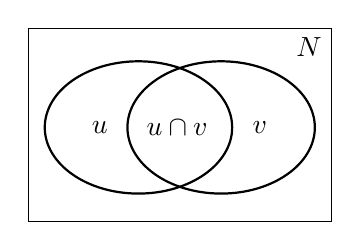
\begin{tikzpicture}[scale=0.7]
  % Rectangle representing N (lighter, not focus)
  \draw[black, thin, opacity=1] (-1.5,-1.5) rectangle (4,2) 
        node[anchor=north east] {$\mathbb{N}$};

  % Set u (ellipse)
  \draw[thick] (0.5,0.2) ellipse (1.7cm and 1.2cm);
  \node at (-0.2,0.2) {$u$};

  % Set v (ellipse)
  \draw[thick] (2.0,0.2) ellipse (1.7cm and 1.2cm);
  \node at (2.7,0.2) {$v$};

  % Intersection label
  \node at (1.2,0.2) {$u \cap v$};
\end{tikzpicture}
\end{center}
\paragraph{Case 2: $v \cap u \ne \emptyset \text{ and } v \subseteq u$.}
Since the sets $v$ and $-u$ are then completely disjoint, $y_{v,G}(\boldsymbol{x}_v)$ is independent of $\boldsymbol{x}_{-u}$ and can be pulled out of the integral:
\[
\int_{\mathbb{R}^{N - |u|}} y_{v,G}(\boldsymbol{x}_v) f_{-u}(\boldsymbol{x}_{-u}) \, d \nu(\boldsymbol{x}_{-u})
= y_{v,G}(\boldsymbol{x}_v) \int_{\mathbb{R}^{N - |u|}} f_{-u}(\boldsymbol{x}_{-u}) \, d \nu(\boldsymbol{x}_{-u})
= y_{v,G}(\boldsymbol{x}_v),
\]
which works because $f_{-u}$ integrates to one.
\begin{center}
    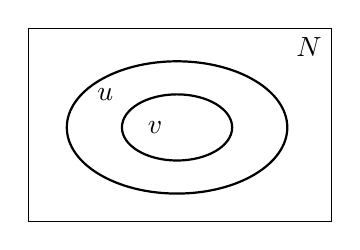
\begin{tikzpicture}[scale=0.7]
  % Rectangle for N (light, not focus)
  \draw[black, thin, opacity=1] (-1.5,-1.5) rectangle (4,2) 
        node[anchor=north east] {$\mathbb{N}$};

  % Set u (outer ellipse)
  \draw[thick] (1.2,0.2) ellipse (2.0cm and 1.2cm);
  \node at (-0.1,0.8) {$u$};

  % Set v (nested inside)
  \draw[thick] (1.2,0.2) ellipse (1.0cm and 0.6cm);
  \node at (0.8,0.2) {$v$};
\end{tikzpicture}
\end{center}
\paragraph{Case 3: \( v \cap u = \emptyset \).}
In this case, we have \( v \subseteq -u \), so \( v \cap -u = v \). Thus, \citet{rahman2014} writes:
\[
\begin{aligned}
\int_{\mathbb{R}^{N - |u|}} y_{v,G}(\boldsymbol{x}_v) f_{-u}(\boldsymbol{x}_{-u}) \, d \nu(\boldsymbol{x}_{-u})
&= \int_{\mathbb{R}^{|v|}} y_{v,G}(\boldsymbol{x}_v)
\left( \int_{\mathbb{R}^{N - |u| - |v|}} f_{-u}(\boldsymbol{x}_{-u}) \, d \nu(\boldsymbol{x}_{-u \setminus v}) \right)
d \nu(\boldsymbol{x}_v) \\[3ex]
&= \int_{\mathbb{R}^{|v|}} y_{v,G}(\boldsymbol{x}_v) f_v(\boldsymbol{x}_v) \, d \nu(\boldsymbol{x}_v) \\[3ex]
&= \int_{\mathbb{R}^{|v|-1}} \left( \int_{\mathbb{R}} y_{v,G}(\boldsymbol{x}_v) f_v(\boldsymbol{x}_v) \, d \nu(x_i) \right)
\prod_{\substack{j \in v \\ j \ne i}} d \nu (x_j) \\
&= 0,
\end{aligned}
\]
while the integral is split in such a way that one recognizes the marginal density $f_v$, and we employ the zero-mean property.
\begin{center}
    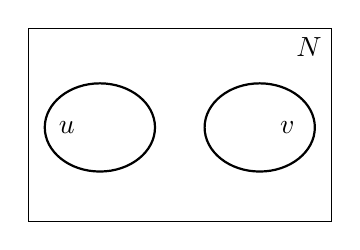
\begin{tikzpicture}[scale=0.7]
  % Rectangle for N (lighter, not focus)
  \draw[black, thin, opacity=1] (-1.5,-1.5) rectangle (4,2)
        node[anchor=north east] {$\mathbb{N}$};

  % Set u (left, ellipse)
  \draw[thick] (-0.2,0.2) ellipse (1cm and 0.8cm);
  \node at (-0.8,0.2) {$u$};

  % Set v (right, ellipse, disjoint from u)
  \draw[thick] (2.7,0.2) ellipse (1cm and 0.8cm);
  \node at (3.2,0.2) {$v$};

  % Example index i inside v (optional)
  % \node at (2.5,-0.2) {$i$};
\end{tikzpicture}
\end{center}
\end{proof}
As we will see in the following, we will encounter all of these three integration cases from \autoref{prop:generalized_fanova_integration_cases} in the definition of the generalized fANOVA components à la \cite{rahman2014}.
In \autoref{prop:generalized_fanova_integration_cases} we also already see that the smartly chosen probability density function is $f_{-u}(\boldsymbol{x}_{-u})$.
\begin{proposition}\label{prop:generalized_fanova_components_rahman}
The generalized fANOVA component functions \( y_{u,G}(\boldsymbol{x}_u), u \subseteq \{1,\dots,N\} \) of a square-integrable function $y:\mathbb{R}^N \to \mathbb{R}$ for a given probability measure $f_{\boldsymbol{X}}(\boldsymbol{x}) d\nu(\boldsymbol{x})$ of $\boldsymbol{X} \in \mathbb{R}^N$ can be recursively defined via the following set of equations:
\begin{align}
y_{\emptyset,G} &= \int_{\mathbb{R}^N} y(\boldsymbol{x}) f_{\boldsymbol{X}}(\boldsymbol{x}) \, d \nu(\boldsymbol{x}) \\[3ex]
y_{u,G}(\boldsymbol{X}_u) &= \int_{\mathbb{R}^{N - |u|}} y(\boldsymbol{X}_u, \boldsymbol{x}_{-u}) f_{-u}(\boldsymbol{x}_{-u}) \, d \nu(\boldsymbol{x}_{-u})
- \sum_{v \subsetneq u} y_{v,G}(\boldsymbol{X}_v) \notag \\
&\quad - \sum_{\substack{\emptyset \ne v \subseteq \{1,\dots,N\} \\ v \cap u \ne \emptyset,\ v \not\subset u}} 
\int_{\mathbb{R}^{|v \cap -u|}} y_{v,G}(\boldsymbol{X}_{v \cap u}, \boldsymbol{x}_{v \cap -u}) f_{v \cap -u}(\boldsymbol{x}_{v \cap -u}) \, d \nu(\boldsymbol{x}_{v \cap -u}).
\end{align}
\end{proposition}
\begin{proof}
\citet{rahman2014} begins by integrating both sides of the generalized fANOVA decomposition
\[
y(\boldsymbol{x}) = \sum_{v \subseteq \{1,\dots,N\}} y_{v,G}(\boldsymbol{x}_v)
\]
w.r.t. $f_{-u}(\boldsymbol{x}_{-u})\, d \nu(\boldsymbol{x}_{-u})$, replacing $\boldsymbol{X}$ by $\boldsymbol{x}$, and changing the dummy index from $u$ to $v$. This yields:
\[
\int_{\mathbb{R}^{N - |u|}} y(\boldsymbol{x}) f_{-u}(\boldsymbol{x}_{-u}) \, d \nu(\boldsymbol{x}_{-u})
= \sum_{v \subseteq \{1,\dots,N\}} \int_{\mathbb{R}^{N - |u|}} y_{v,G}(\boldsymbol{x}_v) f_{-u}(\boldsymbol{x}_{-u}) \, d \nu(\boldsymbol{x}_{-u}).
\]
\paragraph{Case: \( u = \emptyset \).}
We set $u = \emptyset$, so $-u = \{1,\dots,N\}$ and $f_{-u}(\boldsymbol{x}_{-u}) d \nu(\boldsymbol{x}_{-u}) = f_{\boldsymbol{X}}(\boldsymbol{x}) d \nu(\boldsymbol{x})$. The above integral can then be written as:
\[
\int_{\mathbb{R}^N} y(\boldsymbol{x}) f_{\boldsymbol{X}}(\boldsymbol{x}) \, d \nu(\boldsymbol{x})
= \sum_{v \subseteq \{1,\dots,N\}} \int_{\mathbb{R}^N} y_{v,G}(\boldsymbol{x}_v) f_{\boldsymbol{X}}(\boldsymbol{x}) \, d \nu(\boldsymbol{x})
\]
\[
= y_{\emptyset,G}
+ \sum_{\emptyset \ne v \subseteq \{1,\dots,N\}} \int_{\mathbb{R}^N} y_{v,G}(\boldsymbol{x}_v) f_{\boldsymbol{X}}(\boldsymbol{x}) \, d \nu(\boldsymbol{x})
\]
\[
= y_{\emptyset,G} + \sum_{\emptyset \ne v \subseteq \{1,\dots,N\}} \mathbb{E}[y_{v,G}(\boldsymbol{X}_v)] = y_{\emptyset,G},
\]
where the last sum vanishes given the weak annihilating conditions are satisfied.

\paragraph{Case: \( \emptyset \ne u \subseteq \{1,\dots,N\} \).}
Returning to the integrated decomposition
\[
\int_{\mathbb{R}^{N - |u|}} y(\boldsymbol{x}) f_{-u}(\boldsymbol{x}_{-u}) \, d \nu(\boldsymbol{x}_{-u})
= \sum_{v \subseteq \{1,\dots,N\}} \int_{\mathbb{R}^{N - |u|}} y_{v,G}(\boldsymbol{x}_v) f_{-u}(\boldsymbol{x}_{-u}) \, d \nu(\boldsymbol{x}_{-u}),
\]
and applying \autoref{prop:generalized_fanova_integration_cases} to evaluate each term in the sum according to the relationship between $v$ and $u$ yields four cases:

\begin{itemize}
  \item[\textbf{(A)}] \( v \cap u \ne \emptyset \) and \( v \not\subset u \): \\
  This corresponds to case 1 of \autoref{prop:generalized_fanova_integration_cases}. The integral becomes:
  \[
  \sum_{\substack{\emptyset \ne v \subseteq \{1,\dots,N\} \\ v \cap u \ne \emptyset,\ v \not\subset u}} 
  \int_{\mathbb{R}^{|v \cap -u|}} y_{v,G}(\boldsymbol{x}_v) f_{v \cap -u}(\boldsymbol{x}_{v \cap -u}) \, d \nu(\boldsymbol{x}_{v \cap -u}).
  \]

  \item[\textbf{(B)}] \( v \subsetneq u \): \\
  This is contained in case 2 of \autoref{prop:generalized_fanova_integration_cases}. The integrals reduce to the component functions themselves:
  \[
  \sum_{v \subsetneq u} y_{v,G}(\boldsymbol{x}_v).
  \]

  \item[\textbf{(C)}] \( v = u \): \\
  This is also contained in case 2 of \autoref{prop:generalized_fanova_integration_cases}. The integral becomes:
  \[
  y_{u,G}(\boldsymbol{x}_u).
  \]

  \item[\textbf{(D)}] \( v \cap u = \emptyset \): \\
  This is case 3 of \autoref{prop:generalized_fanova_integration_cases}, therefore these terms vanish:
  \[
  \sum_{\substack{v \subseteq \{1,\dots,N\} \\ v \cap u = \emptyset}} 0 = 0.
  \]
\end{itemize}
Putting everything together:
\[
\begin{aligned}
&\int_{\mathbb{R}^{N - |u|}} y(\boldsymbol{x}) f_{-u}(\boldsymbol{x}_{-u}) 
    \, d \nu(\boldsymbol{x}_{-u}) \\
&= y_{u,G}(\boldsymbol{x}_u)
   + \sum_{v \subsetneq u} y_{v,G}(\boldsymbol{x}_v) + 
   \sum_{\substack{\emptyset \ne v \subseteq \{1,\dots,N\} \\
                   v \cap u \ne \emptyset,\ v \not\subset u}} 
   \int_{\mathbb{R}^{|v \cap -u|}} 
        y_{v,G}(\boldsymbol{x}_v) 
        f_{v \cap -u}(\boldsymbol{x}_{v \cap -u}) 
        \, d \nu(\boldsymbol{x}_{v \cap -u}).
\end{aligned}
\]
Rearranging gives the almost final expression for \( y_{u,G}(\boldsymbol{x}_u) \):
\[
\begin{aligned}
y_{u,G}(\boldsymbol{x}_u)
&= 
\int_{\mathbb{R}^{N - |u|}} 
    y(\boldsymbol{x}) 
    f_{-u}(\boldsymbol{x}_{-u}) 
    \, d \nu(\boldsymbol{x}_{-u})
\\[0.5em]
&\quad
- \sum_{v \subsetneq u} 
    y_{v,G}(\boldsymbol{x}_v)
\\[0.5em]
&\quad
- \sum_{\substack{\emptyset \ne v \subseteq \{1,\dots,N\}\\
                    v \cap u \ne \emptyset,\ v \not\subset u}}
    \int_{\mathbb{R}^{|v \cap -u|}} 
        y_{v,G}(\boldsymbol{x}_v) 
        f_{v \cap -u}(\boldsymbol{x}_{v \cap -u}) 
        \, d \nu(\boldsymbol{x}_{v \cap -u}).
\end{aligned}
\]


As a final step, \citet{rahman2014} writes \( v = (v \cap u) \cup (v \cap -u) \) to obtain the expression of \autoref{prop:generalized_fanova_components_rahman}.
\end{proof}

% Alternative definition of components by Hooker
\subsubsection{Generalization via Projection}
\cite{hooker2007} approaches his generalization of the fANOVA decomposition from the angle of orthogonal projections. Instead of the more recursive definition of the components functions as in \cite{rahman2014}, he defines the fANOVA components as a joint set which simultaneously minimizes the squared difference to the original function $y$ under certain constraints.
The constraints he sets for the optimization problem should ensure that the generalized components satisfy the desired properties of zero-mean and hierarchical orthogonality.
The generalized fANOVA component functions $\{y_u(x_u) | u \subseteq d \}$ jointly satisfy:
\begin{equation}
\left\{ y_{u, G}(\boldsymbol{x}_u) \,\middle|\, u \subseteq d \right\}
= \arg\min_{\{g_u \in \mathcal{L}^2(\mathbb{R}^{|u|})\}} 
\int_{\mathbb{R}^N} \left( \sum_{u \subseteq d} g_u(\boldsymbol{x}_u) - y(\boldsymbol{x}) \right)^2 f_{\boldsymbol{X}}(\boldsymbol{x}) \, d \nu (\boldsymbol{x})
\label{eq:generalized_fanova_components_hooker}
\end{equation}
under the hierarchical orthogonality conditions:
\begin{equation}
    \forall v \subseteq u,\ \forall g_v : \int_{\mathbb{R}^N} y_u(\boldsymbol{x}_u) g_v(\boldsymbol{x}_v) f_{\boldsymbol{X}}(\boldsymbol{x}) \, d \nu (\boldsymbol{x}) = 0.
\label{eq:hooker_hierarchical_orthogonality}
\end{equation}
In \autoref{eq:generalized_fanova_components_hooker} we recognize a projection. We are simultaneously finding the set of components functions $g_u$ that minimize the weighted squared difference to the original function $y$ (under the given integral constraint), which is exactly the definition of a projection of $y$ onto a specific subspace $\mathcal{G}$ (\autoref{def:orthogonal_projection}).\par
However, the constraint in \autoref{eq:hooker_hierarchical_orthogonality} is infeasible to enforce in practice. 
Therefore, Hooker formulated the following proposition, which ensures hierarchical orthogonality of the fANOVA components and thus forms the building block of his approach. It can be compared to the weak annihilating conditions (\autoref{cond:weak_annihilating_conditions}) in \cite{rahman2014}.
\begin{proposition}
    The hierarchical orthogonality of the fANOVA components is ensured if and only if the following integral condition holds:
    \begin{equation}
\forall u \subseteq N,\ \forall i \in u:\ \int_{\mathbb{R}^N} y_u(\boldsymbol{x}_u) f_{\boldsymbol{X}}(\boldsymbol{x})\, d \nu (x_i)\, d \nu (\boldsymbol{x}_{-u}) = 0.
\end{equation}
\label{prop:hooker_lemma_1}
\end{proposition}
\begin{proof}
    The proof is organized in two parts. First, Hooker shows that, the hierarchical orthogonality is true, if the integral conditions hold. Second, he shows that hierarchical orthogonality breaks down if the integral conditions are not true.\par
    For the first part, assume that \autoref{prop:hooker_lemma_1} holds. Let $i \in u \setminus v$, then $y_v(\boldsymbol{x}_v)$ is independent of $x_i$ and $\boldsymbol{x}_{-u}$, so we can write:
\begin{align*}
\langle y_u, y_v \rangle 
&:= \int_{\mathbb{R}^N} 
        y_v(\boldsymbol{x}_v)\, y_u(\boldsymbol{x}_u)\, 
        f_{\boldsymbol{X}}(\boldsymbol{x})\, 
        d \nu(\boldsymbol{x}) \\[0.3em]
&= y_v(\boldsymbol{x}_v) 
   \int_{\mathbb{R}^N} 
        y_u(\boldsymbol{x}_u)\, 
        f_{\boldsymbol{X}}(\boldsymbol{x})\, 
        d \nu(\boldsymbol{x}) \\[0.3em]
&= 0.
\end{align*}
For the second part, assume that there exists a subset $u$ and an index $i$ for which hierarchical orthogonality does not hold, i.e.
\begin{equation*}
    \int_{\mathbb{R}^N} y_u(\boldsymbol{x}_u)\, f_{\boldsymbol{X}}(\boldsymbol{x})\, d \nu (x_i)\, d \nu (x_{-u}) \ne 0 
    \quad \text{for some} \quad i, u.
\end{equation*}
Further, assume that hierarchical orthogonality holds for all subsets $v \neq u$ and indices $j \neq i$. 
Hooker then constructs a fANOVA component function $y_v$ with lower order than $y_u$, which is not orthogonal to $y_u$. 
He sets $v = u \setminus \{i\}$, so $y_v$ is one order lower than $y_u$ and defined as:
\begin{equation*}
    y_v(\boldsymbol{x}_v) := \int_{\mathbb{R}^N} f_u(\boldsymbol{x}_u) \, f_{\boldsymbol{X}}(\boldsymbol{x}) \, d \nu (x_i) \, d \nu (\boldsymbol{x}_{-u}).
\end{equation*}
$y_v$ is a valid fANOVA component, which is unequal to zero by assumption of hierarchical orthogonality being false, while it itself satisfies hierarchical orthogonality by assumption:
\begin{equation*}
    \forall j \in v, \quad \int_{\mathbb{R}^N} y_v(\boldsymbol{x}_v) \, f_{\boldsymbol{X}}(\boldsymbol{x}) \, d \nu (x_j) \, d \nu (\boldsymbol{x}_{-v}) = 0.
\end{equation*}
Hooker then shows that $y_v$ is not orthogonal to $y_u$:
\begin{align*}
    \langle y_u, y_v \rangle
        &= \int_{\mathbb{R}^N} y_u(\boldsymbol{x}_u) \, y_v(\boldsymbol{x}_v) \, f_X(\boldsymbol{x}) \, d \nu(\boldsymbol{x}) \\
        &= \int_{\mathbb{R}^N} y_u(\boldsymbol{x}_u) 
           \left( \int_{\mathbb{R}^N} y_u(\boldsymbol{x}_u) \, f_X(\boldsymbol{x}) \, d \nu(x_i) \, d \nu(\boldsymbol{x}_{-u}) \right) 
           f_{\boldsymbol{X}}(\boldsymbol{x}) \, d \nu(\boldsymbol{x}) \\
        &= \int_{\mathbb{R}^N} 
           \left( \int_{\mathbb{R}^N} y_u(\boldsymbol{x}_u) \, f_X(\boldsymbol{x}) \, d \nu(x_i) \, d \nu(\boldsymbol{x}_{-u}) \right)^2 
           d \nu(\boldsymbol{x}_{u \setminus \{i\}}) \\
        &\neq 0.
\end{align*}
\end{proof}
Hooker approaches his generalization through the lens of projections while Rahman gives a form that tries to imitate the classical fANOVA component functions. A crucial parallel of both versions which distinguishes them from the classical case is that their components are defined in dependence of each other (\autoref{prop:generalized_fanova_components_rahman}, \autoref{prop:generalized_fanova_components_hooker}).
% In the Rahman approach, the components are derived from the original function by integrating out the other variables, while in the Hooker approach, the components are defined through a minimization problem that seeks to best approximate the original function.
This makes it in general difficult to compute the generalized fANOVA component functions analytically, even for simple functions.
\subsubsection{Generalized Variance Decomposition}
Given that the fANOVA decomposition changes under dependent inputs, we briefly make an adjustment to the second-moment statistics of the generalized fANOVA decomposition.
The mean of $y$ remains unchanged and is still given by the constant component \( y_{\emptyset,G} \), i.e.
\[
\mu_G := \mathbb{E}[y(\boldsymbol{X})] = y_{\emptyset,G}.
\]
In contrast, the variance decomposition does not simplify in the same way as \autoref{eq:variance_expansion}, as cross-terms of the same order do not vanish under hierarchical orthogonality.
For $ \emptyset \neq u \subseteq \{1,\dots,N\}$, $\emptyset \neq v \subseteq \{1,\dots,N\}$, $u \neq v$ we restate from above:
\begin{align*}
\sigma^2 
&:= \mathbb{E}\left[ \left( y(\boldsymbol{X}) - \mu_G \right)^2 \right] \notag \\
&= \mathbb{E} \left[ \left( y_{\emptyset,G} + \sum_{u} y_{u,G}(\boldsymbol{X}_u) - y_{\emptyset,G} \right)^2 \right] \notag \\
&= \mathbb{E} \left[ \left( \sum_{u} y_{u,G}(\boldsymbol{X}_u) \right)^2 \right] \notag \\
&= \sum_{u} \mathbb{E} \left[ y_{u,G}^2(\boldsymbol{X}_u) \right]
+ \sum_{\substack{u \not\subseteq v,\, v \not\subseteq u}} 
\mathbb{E} \left[ y_{u,G}(\boldsymbol{X}_u) y_{v,G}(\boldsymbol{X}_v) \right],
\end{align*}
while the first sum in the final line goes over all nonempty subsets $u$ and the second sum goes over all pairs of subsets $(u, v)$ where neither is a subset of the other one.
Conceptually this means that the first term is the sum of the variances of the components, while the second term is the sum of the covariances between components that are not hierarchically orthogonal.
The indices under the second component capture precisely the cross-terms that do not vanish under hierarchical orthogonality. As we saw earlier, cross-terms of the same hierarchy also cancel out under the orthogonality assumption of the classical fANOVA.
\subsubsection{Example: Dependent Multivariate Normal Inputs}
Before ending this section, it remains to answer how the true generalized fANOVA decomposition looks like for our running example. While the interdependence of the generalized components makes it difficult to arrive at an analytical solution, \cite{rahman2014} provides a way to obtain the closed-form solution for any polynomial of maximum two degree under normally distributed input variables.\par
The approach in \cite{rahman2014} is based on a Fourier–polynomial expansion, 
which expresses each generalized fANOVA component functions as a weighted sum of basis functions. 
This shifts the problem from directly determining the components 
to identifying suitable basis functions that can represent the fANOVA component functions. 
Rahman chooses Hermite polynomials as these basis functions because they are, 
by construction, zero-centered and hierarchically orthogonal. 
These properties ensure that the resulting components are also 
zero-centered and hierarchically orthogonal. 
The remaining challenge is then to determine the weights associated with the basis functions, 
which can be obtained through coefficient matching.
A polynomial of degree two has the general form
\begin{align}\label{eq:quadratic_polynomial}
    y(x_1,x_2)
    = a_0 + a_1 x_1 + a_2 x_2 
      + a_{11} x_1^2 + a_{22} x_2^2 + a_{12} x_1 x_2.
\end{align}
Any such polynomial may be expressed as a sum of weighted basis functions of the form \citep{nagler2024linalg}:
\[
\begin{aligned}
y(x_1,x_2)
    &= c_0 
     + c_{1,1}\,\psi_{1,1}(x_1) 
     + c_{2,1}\,\psi_{2,1}(x_2) \\ 
    &\quad
     + c_{1,2}\,\psi_{1,2}(x_1)
     + c_{2,2}\,\psi_{2,2}(x_2) \\
    &\quad
     + c_{12,11}\,\psi_{12,11}(x_1,x_2),
\end{aligned}
\]
where the $\psi_{i,j}$ are the basis functions with corresponding weights 
$c_0, \dots , c_{12,11} \in \mathbb{R}$.
The idea is to carefully construct a set of hierarchically orthogonal basis functions with zero-mean property. Then the expansion in these basis functions is already the 
fANOVA decomposition of a quadratic polynomial, i.e.
\begin{align*}
y(x_1,x_2) 
&= a_0 + a_1 x_1 + a_2 x_2 
   + a_{11} x_1^2 + a_{22} x_2^2 + a_{12} x_1 x_2 \\[3pt]
&= c_0 
   + c_{1,1}\,\psi_{1,1}(x_1) 
   + c_{2,1}\,\psi_{2,1}(x_2) \\[-1pt]
&\quad
   + c_{1,2}\,\psi_{1,2}(x_1)
   + c_{2,2}\,\psi_{2,2}(x_2)
   + c_{12,11}\,\psi_{12,11}(x_1,x_2) \\[3pt]
&= 
   \underbrace{c_0}_{y_0}
   + \underbrace{\big(c_{1,1}\,\psi_{1,1}(x_1) 
                     + c_{1,2}\,\psi_{1,2}(x_1)\big)}_{y_1(x_1)} \\[-1pt]
&\quad
   + \underbrace{\big(c_{2,1}\,\psi_{2,1}(x_2) 
                     + c_{2,2}\,\psi_{2,2}(x_2)\big)}_{y_2(x_2)} \\[-1pt]
&\quad
   + \underbrace{c_{12,11}\,\psi_{12,11}(x_1,x_2)}_{y_{12}(x_1,x_2)}.
\end{align*}
Derived from the probability density of a multivariate normal distribution, \cite{rahman2014} chooses multivariate Hermite polynomials. We use a slightly simplified version of the proposed basis functions to find an explicit solution for our running example\footnote{We omit the scaling factor, which means the basis functions are not orthonormal anymore but still orthogonal.}. The basis functions we work with are:
\[
\begin{aligned}
\psi_{\emptyset}(x_1,x_2) &= 1, \\[3pt]
\psi_{1,1}(x_1) &= x_1, \\[3pt]
\psi_{2,1}(x_2) &= x_2, \\[3pt]
\psi_{1,2}(x_1) &= x_1^2 - 1, \\[3pt]
\psi_{2,2}(x_2) &= x_2^2 - 1, \\[3pt]
\psi_{12,11}(x_1,x_2) &= \frac{\rho (x_1^2 + x_2^2)}{1 + \rho^2} 
                         - x_1 x_2 
                         + \frac{\rho(\rho^2 - 1)}{1 + \rho^2},
\end{aligned}
\]
where $\rho$ is the correlation coefficient between $X_1$ and $X_2$. So this formula will work for dependent as well as independent inputs.\par
% --- Model decomposition (general coefficients) ---
What remains it to find the coefficients $c_0, c_{1,1}, \dots, c_{12, 11}$ such that the weighted sum of the basis functions truly recovers the original polynomial in \autoref{eq:quadratic_polynomial}.
To find the correct weights, we substitute the basis functions and rearrange terms to recognize the groups more easily:
\begin{align*}
% --- Original polynomial ---
y(x_1,x_2) &= c_0 + c_{1,1} x_1 + c_{2,1} x_2 
+ c_{1,2}(x_1^2 - 1) + c_{2,2}(x_2^2 - 1) \notag \\[3pt]
&\quad + c_{12, 11}\left( \frac{\rho(x_1^2 + x_2^2)}{1 + \rho^2} 
- x_1 x_2 
+ \frac{\rho(\rho^2 - 1)}{1 + \rho^2} \right) \\[3pt]
% --- Collecting like terms ---
&= 
\big( c_0 - c_{1,2} - c_{2,2} + c_{12, 11}\,\tfrac{\rho(\rho^2 - 1)}{1+\rho^2} \big)
+ c_{1,1}\,x_1 
+ c_{2,1}\,x_2 \notag \\[3pt]
&\quad + \big( c_{1,2} + c_{12, 11}\,\tfrac{\rho}{1+\rho^2} \big) x_1^2
+ \big( c_{2,2} + c_{12, 11}\,\tfrac{\rho}{1+\rho^2} \big) x_2^2
- c_{12, 11}\, x_1 x_2.
\end{align*}
Now we can use monomial matching to find the coefficients. It is best to start with the interaction term and work backwards from there to the constant term, plugging in the current solutions along the way:
% --- Monomial matching equations ---
\begin{align*}
-\,c_{12, 11} &= a_{12} &\Rightarrow\quad c_{12, 11} &= -a_{12} \\[3pt]
c_{1,2} + c_{12, 11}\,\tfrac{\rho}{1+\rho^2} &= a_{11} 
&\Rightarrow\quad c_{1,2} &= a_{11} + \tfrac{\rho}{1+\rho^2}a_{12} \\[3pt]
c_{2,2} + c_{12, 11}\,\tfrac{\rho}{1+\rho^2} &= a_{22} 
&\Rightarrow\quad c_{2,2} &= a_{22} + \tfrac{\rho}{1+\rho^2}a_{12} \\[3pt]
c_{1,1} &= a_1 \\[3pt]
c_{2,1} &= a_2 \\[3pt]
c_0 - c_{1,2} - c_{2,2} + c_{12, 11}\,\tfrac{\rho(\rho^2 - 1)}{1+\rho^2} &= a_0 
&\Rightarrow\quad 
c_0 &= a_0 + a_{11} + a_{22} + \rho\,a_{12}
\end{align*}

Hence, the generalized fANOVA decomposition of a two-degree polynomial is given by:
\begin{align*}
y(x_1,x_2) 
&= c_0 
  + c_{1,1}\,\psi_{1,1}(x_1) 
  + c_{2,1}\,\psi_{2,1}(x_2) \\
&+ c_{1,2}\,\psi_{1,2}(x_1)
  + c_{2,2}\,\psi_{2,2}(x_2)
  + c_{12,11}\,\psi_{12,11}(x_1,x_2) \\[5pt]
&= 
\underbrace{\big(a_0 + a_{11} + a_{22} + \rho\,a_{12}\big)}_{c_0} 
+ \underbrace{a_1}_{c_{1,1}} x_1
+ \underbrace{a_2}_{c_{2,1}} x_2 \\ 
&\quad 
+ \underbrace{\left(a_{11} + \frac{\rho}{1+\rho^2}a_{12}\right)}_{c_{1,2}} (x_1^2 - 1)
+ \underbrace{\left(a_{22} + \frac{\rho}{1+\rho^2}a_{12}\right)}_{c_{2,2}} (x_2^2 - 1) \notag \\
&\quad 
+ \underbrace{(-a_{12})}_{c_{12, 11}}\left(
    \frac{\rho(x_1^2+x_2^2)}{1+\rho^2} - x_1 x_2 
    + \frac{\rho(\rho^2-1)}{1+\rho^2}
  \right) \\[5pt]
&= 
(a_0 + a_{11} + a_{22} + \rho a_{12})
+ a_1 x_1
+ a_2 x_2 \notag \\ 
&\quad 
+ \left(a_{11} + \frac{\rho}{1+\rho^2} a_{12}\right)(x_1^2 - 1)
+ \left(a_{22} + \frac{\rho}{1+\rho^2} a_{12}\right)(x_2^2 - 1) \notag \\
&\quad 
- a_{12}\left(
  \frac{\rho(x_1^2 + x_2^2)}{1+\rho^2}
  - x_1 x_2
  + \frac{\rho(\rho^2 - 1)}{1+\rho^2}
  \right),
\end{align*}
with individual components:
\begin{align}
\begin{split}
y_{\emptyset} &= a_0 + a_{11} + a_{22} + \rho\,a_{12}, \\[3pt]
y_{\{1\}}(x_1) &= a_1\,x_1 
  + \left(a_{11} + \frac{\rho}{1+\rho^2}a_{12}\right)\bigl(x_1^2 - 1\bigr), \\[3pt]
y_{\{2\}}(x_2) &= a_2\,x_2 
  + \left(a_{22} + \frac{\rho}{1+\rho^2}a_{12}\right)\bigl(x_2^2 - 1\bigr), \\[3pt]
y_{\{1,2\}}(x_1,x_2) 
&= -a_{12}\!\left(
    \frac{\rho(x_1^2+x_2^2)}{1+\rho^2} 
    - x_1 x_2 
    + \frac{\rho(\rho^2-1)}{1+\rho^2}
   \right).
\end{split}
\label{eq:fanova_components_2D_polynomial}
\end{align}
This set of component functions is true under the assumption of Gaussian inputs. The basis representation is still correct for other distribution assumptions in the sense that it recovers the original function; however, the component function would not be hierarchically orthogonal anymore.\par
With this we are able to give the fANOVA component functions for our running example in a generalized form, which allows for dependent input variables, assumed to be Gaussian.\par
For $h(x_1,x_2) = x_1 + 2x_2 + x_1 x_2$  we have $a_0 = 0, a_1 = 1, a_2 = 2, a_{11} = 0, a_{22} = 0, a_{12} = 1$, and therefore obtain with \autoref{eq:fanova_components_2D_polynomial}:
\begin{align*}
h_{\emptyset} &= \rho, \\[3pt]
h_{\{1\}}(x_1) &= x_1 + \frac{\rho}{1+\rho^2}(x_1^2 - 1), \\[3pt]
h_{\{2\}}(x_2) &= 2\,x_2 + \frac{\rho}{1+\rho^2}(x_2^2 - 1), \\[3pt]
h_{\{1,2\}}(x_1,x_2) 
&= -\left(\frac{\rho(x_1^2+x_2^2)}{1+\rho^2} - x_1 x_2 + \frac{\rho(\rho^2-1)}{1+\rho^2}\right).
\end{align*}

% Let us come back to our example from the beginning. The goal is to write
% \[
% g(x_1, x_2) = y_{\emptyset, G} + y_{1, G}(x_1) + y_{2, G}(x_2) + y_{1,2, G}(x_1, x_2)
% \]
% under dependent inputs. It turns out that finding the generalized fANOVA components analytically is quite challenging. We present two ways in which the problem solution can be stated.\par

% \subsubsection*{Rahman method}
% The system to find the generalized fANOVA components for $g$ according to \cite{rahman2014} method looks as follows:
% \begin{align*}
%     y_{\emptyset, G} &= \int_{\mathbb{R}^2} g(x_1, x_2)\, f(x_1, x_2)\, dx_1 dx_2 \\
%     y_{1, G}(x_1) &= \int_{\mathbb{R}} g(x_1, x_2)\, f_2(x_2)\, dx_2
%     - y_{\emptyset, G}
%     - \int_{\mathbb{R}} y_{\{1,2\}, G}(x_1, x_2)\, f_2(x_2)\, dx_2\\
%     y_{2, G}(x_2) &= \int_{\mathbb{R}} g(x_1, x_2)\, f_1(x_1)\, dx_1
%     - y_{\emptyset, G}
%     - \int_{\mathbb{R}} y_{\{1,2\}, G}(x_1, x_2)\, f_1(x_1)\, dx_1\\
%     y_{1,2, G}(x_1, x_2) &= g(x_1, x_2) - y_{\emptyset, G} - y_{\{1\}, G}(x_1) - y_{\{2\}, G}(x_2)
% \end{align*}

% Since the components form a coupled system where the components are defined in interdependence of each other, finding the solution is not straight forward, even for simple examples.

% \subsubsection*{Hooker method}
% An alternative way to phrase the problem can be found in \cite{hooker2007}.
% To find the generalized fANOVA components, we can formulate a minimization problem for each of them. 
% \begin{align*}
% y_{\emptyset} 
% &= \arg\min_{c \in \mathbb{R}} \int_{\mathbb{R}^2} 
% \left( g(x_1, x_2) 
% - \left( c + y_{\{1\}}(x_1) + y_{\{2\}}(x_2) + y_{\{1,2\}}(x_1, x_2) \right) \right)^2 
% f(x_1, x_2)\, dx_1 dx_2 \\[1em]
% y_{1}(x_1) 
% &= \arg\min_{h_1 \in L^2(\mathbb{R})} \int_{\mathbb{R}^2} 
% \left( g(x_1, x_2) 
% - \left( y_{\emptyset} + h_1(x_1) + y_{\{2\}}(x_2) + y_{\{1,2\}}(x_1, x_2) \right) \right)^2 
% f(x_1, x_2)\, dx_1 dx_2 \\[1em]
% y_{2}(x_2) 
% &= \arg\min_{h_2 \in L^2(\mathbb{R})} \int_{\mathbb{R}^2} 
% \left( g(x_1, x_2) 
% - \left( y_{\emptyset} + y_{\{1\}}(x_1) + h_2(x_2) + y_{\{1,2\}}(x_1, x_2) \right) \right)^2 
% f(x_1, x_2)\, dx_1 dx_2 \\[1em]
% y_{1,2}(x_1, x_2) 
% &= \arg\min_{h_{12} \in L^2(\mathbb{R}^2)} \int_{\mathbb{R}^2} 
% \left( g(x_1, x_2) 
% - \left( y_{\emptyset} + y_{\{1\}}(x_1) + y_{\{2\}}(x_2) + h_{12}(x_1, x_2) \right) \right)^2 
% f(x_1, x_2)\, dx_1 dx_2
% \end{align*}



% The least-squares problems are solved subject to the following constraints, which ensure that the resulting components are zero centred and hierarchically orthogonal:
% \begin{align*}
% \int_{\mathbb{R}^2} y_{\{1\}}(x_1) \cdot f(x_1, x_2)\, dx_1 dx_2 &= 0 \\[1ex]
% \int_{\mathbb{R}^2} y_{\{2\}}(x_2) \cdot f(x_1, x_2)\, dx_1 dx_2 &= 0 \\[1.4ex]
% \int_{\mathbb{R}} y_{\{1,2\}}(x_1, x_2) \cdot f(x_1, x_2)\, dx_1 &= 0 \quad \forall x_2 \\[1ex]
% \int_{\mathbb{R}} y_{\{1,2\}}(x_1, x_2) \cdot f(x_1, x_2)\, dx_2 &= 0 \quad \forall x_1
% \end{align*}


% Conceptually \cite{hooker2007} is doing nothing other than a projection. Earlier, we established that a projection is the same as the conditional expected value, and fANOVA can be expressed via the conditional expected value. This means from the initial idea, we do not change anything apart from the fact that we have to integrate via the joint pdf, but this is something one is ``forced'' to under dependence, not something one ``invents''. However, projections onto subspaces become more difficult under dependence; therefore, setting these constraints explicitly is necessary to ensure (hierarchical) orthogonality.\par
% Obtaining an analytical solution for either of the methods is tedious even for our simple example. We leave it at the problem formulation, so that we have the comparison between which problem one has to solve the classical case versus the generalized case. In the next section, we sketch ways to estimate the fANOVA components conceptually.



